\documentclass[11pt,letterpaper]{article}

\usepackage[T1]{fontenc}
\usepackage{lmodern}
\usepackage[margin=0.85in,headheight=22pt]{geometry}
\usepackage[table]{xcolor}
\usepackage{amsmath,amssymb,mathtools}
\usepackage{booktabs,array,tabularx,longtable,multirow}
\usepackage{enumitem}
\usepackage{microtype}
\usepackage{graphicx}
\usepackage{tikz}
\usetikzlibrary{arrows.meta,positioning,shapes.geometric,fit,calc}
\usepackage[most]{tcolorbox}
\usepackage{fancyhdr}
\usepackage{titlesec}
\usepackage{pdflscape}
\usepackage{hyperref}

\definecolor{navy}{HTML}{17324D}
\definecolor{blue}{HTML}{2D6381}
\definecolor{teal}{HTML}{34766F}
\definecolor{ink}{HTML}{25313A}
\definecolor{muted}{HTML}{5E6B75}
\definecolor{line}{HTML}{CBD5DB}
\definecolor{paper}{HTML}{F5F7F8}
\definecolor{paleBlue}{HTML}{EAF1F5}
\definecolor{paleGreen}{HTML}{EAF4EF}
\definecolor{paleAmber}{HTML}{F7F1E7}

\hypersetup{
  colorlinks=true,
  linkcolor=blue,
  citecolor=teal,
  urlcolor=blue,
  pdftitle={Understanding Hypergraph-Product qLDPC Codes and Decoding},
  pdfauthor={qLDPC CoDesign Explorer},
  pdfsubject={Technical learning and implementation guide}
}

\pagestyle{fancy}
\fancyhf{}
\fancyhead[L]{\small\color{muted}qLDPC CoDesign Explorer}
\fancyhead[R]{\small\color{muted}HGP and Decoding Guide}
\fancyfoot[C]{\small\color{muted}\thepage}
\renewcommand{\headrulewidth}{0.4pt}
\renewcommand{\headrule}{\hbox to\headwidth{\color{line}\leaders\hrule height \headrulewidth\hfill}}

\titleformat{\section}{\Large\bfseries\color{navy}}{\thesection}{0.65em}{}
\titleformat{\subsection}{\large\bfseries\color{navy}}{\thesubsection}{0.65em}{}
\titleformat{\subsubsection}{\normalsize\bfseries\color{ink}}{\thesubsubsection}{0.65em}{}
\titlespacing*{\section}{0pt}{2.1em}{0.8em}
\titlespacing*{\subsection}{0pt}{1.5em}{0.55em}

\setlength{\parindent}{0pt}
\setlength{\parskip}{0.62em}
\setlist[itemize]{leftmargin=1.4em,itemsep=0.28em,topsep=0.35em}
\setlist[enumerate]{leftmargin=1.55em,itemsep=0.35em,topsep=0.35em}
\renewcommand{\arraystretch}{1.22}

\newcommand{\F}{\mathbb{F}_2}
\newcommand{\wt}{\operatorname{wt}}
\newcommand{\rank}{\operatorname{rank}}
\newcommand{\rowspan}{\operatorname{rowspan}}
\newcommand{\cmark}{\ensuremath{\checkmark}}
\newcommand{\code}[1]{\texttt{#1}}

\newtcolorbox{keyidea}[1][Key idea]{
  enhanced,
  colback=paleBlue,
  colframe=blue,
  coltitle=navy,
  fonttitle=\bfseries,
  title=#1,
  boxrule=0.7pt,
  arc=2mm,
  left=3mm,right=3mm,top=2mm,bottom=2mm
}

\newtcolorbox{projectbox}[1][Project connection]{
  enhanced,
  colback=paleGreen,
  colframe=teal,
  coltitle=navy,
  fonttitle=\bfseries,
  title=#1,
  boxrule=0.7pt,
  arc=2mm,
  left=3mm,right=3mm,top=2mm,bottom=2mm
}

\newtcolorbox{warningbox}[1][Common pitfall]{
  enhanced,
  colback=paleAmber,
  colframe=orange!65!black,
  coltitle=ink,
  fonttitle=\bfseries,
  title=#1,
  boxrule=0.7pt,
  arc=2mm,
  left=3mm,right=3mm,top=2mm,bottom=2mm
}

\begin{document}

\begin{titlepage}
  \pagecolor{navy}
  \color{white}
  \vspace*{0.65in}
  {\Large\bfseries qLDPC CoDesign Explorer\par}
  \vspace{0.18in}
  {\color{white!65}\rule{\textwidth}{0.7pt}\par}
  \vspace{0.75in}
  {\fontsize{26}{32}\selectfont\bfseries Understanding Hypergraph-Product\\qLDPC Codes and Decoding\par}
  \vspace{0.3in}
  {\Large A technical learning and implementation guide\par}
  \vspace{0.55in}

  \begin{tcolorbox}[
    colback=navy!78!black,
    colframe=white!25,
    coltext=white!92,
    boxrule=0.6pt,
    arc=2mm,
    left=5mm,right=5mm,top=4mm,bottom=4mm
  ]
  \color{white!92}
  This guide builds one connected mental model from binary parity checks to CSS stabilizers,
  hypergraph-product construction, syndrome extraction, and qLDPC decoding. It also maps each
  concept to the planned Configure, Inject, Observe, and Decode workflow of the project.
  \end{tcolorbox}

  \vfill
  \begin{tabular}{@{}ll@{}}
    \color{white!60}Document version & \color{white}1.0 \\
    \color{white!60}Date & \color{white}September 2026 \\
    \color{white!60}Scope & \color{white}qLDPC and hypergraph-product codes only \\
    \color{white!60}Starting noise model & \color{white}Code-capacity Pauli noise \\
  \end{tabular}
  \vspace{0.3in}
\end{titlepage}
\nopagecolor

\begin{tcolorbox}[colback=paper,colframe=line,boxrule=0.6pt,arc=2mm]
\textbf{How to use this guide.} Chapters 1--5 establish the mathematics. Chapters 6--9 explain
errors, syndromes, and decoding in operational terms. Chapters 10--12 turn those ideas into the
software and experimental plan for the explorer. The appendices provide notation, explicit
matrices for the project fixture, and implementation checklists.
\end{tcolorbox}

\tableofcontents
\clearpage

\section{Learning goals and project scope}

By the end of this guide, a reader should be able to:

\begin{itemize}
  \item explain why sparse parity checks are attractive for quantum error correction;
  \item translate between classical parity-check matrices, Tanner graphs, and CSS stabilizers;
  \item construct the two HGP check matrices and verify that they commute;
  \item interpret a Pauli error as two binary vectors and calculate its two syndromes;
  \item state the correct decoding success condition in the presence of degeneracy;
  \item compare exact lookup, belief propagation, BP+OSD, and small-set-flip decoding;
  \item design reproducible qLDPC experiments with honest assumptions and useful metrics; and
  \item understand how these concepts become interactions in the qLDPC CoDesign Explorer.
\end{itemize}

\subsection{The system boundary}

The explorer is intentionally centered on qLDPC codes. It is not a surface-code comparison tool.
The initial teaching fixture is a small HGP code with parameters $[[13,1,3]]$, constructed from two
length-three repetition-code checks. Its small size allows exact verification, explicit matrices,
and complete decoding traces. Later code families can be added behind the same contracts after the
core interactions are trustworthy.

The planned product journey is shown below.

\begin{center}
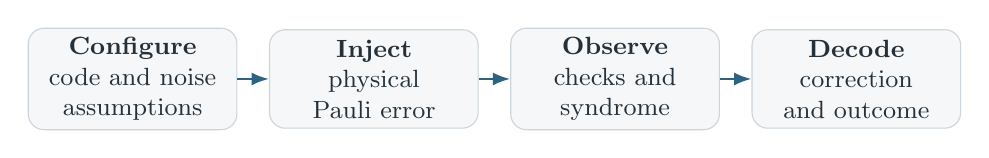
\begin{tikzpicture}[
  node distance=4mm,
  stage/.style={draw=line,rounded corners=2mm,minimum width=2.65cm,text width=2.35cm,minimum height=1.25cm,align=center,fill=paper,text=ink,font=\small},
  arrow/.style={-{Latex[length=2.2mm]},thick,draw=blue}
]
  \node[stage] (c) {\textbf{Configure}\\code and noise assumptions};
  \node[stage,right=of c] (i) {\textbf{Inject}\\physical Pauli error};
  \node[stage,right=of i] (o) {\textbf{Observe}\\checks and syndrome};
  \node[stage,right=of o] (d) {\textbf{Decode}\\correction and outcome};
  \draw[arrow] (c) -- (i);
  \draw[arrow] (i) -- (o);
  \draw[arrow] (o) -- (d);
\end{tikzpicture}
\end{center}

Each stage should expose a state transition that can be inspected and reproduced. The interface
should never imply that a decoder succeeded merely because it returned a vector.

\section{From classical parity checks to LDPC structure}

\subsection{Binary linear codes}

A binary linear code is a vector subspace $C\subseteq\F^n$. A parity-check matrix
$H\in\F^{m\times n}$ defines the code as
\begin{equation}
  C=\ker H=\{c\in\F^n: Hc^{\mathsf T}=0\}.
\end{equation}
If $r=\rank(H)$, then the number of encoded classical bits is $k=n-r$. The code distance is the
minimum Hamming weight of a nonzero codeword,
\begin{equation}
  d=\min_{c\in C\setminus\{0\}}\wt(c).
\end{equation}

If a codeword is corrupted by an error $e\in\F^n$, the receiver observes the syndrome
\begin{equation}
  s=He^{\mathsf T}.
\end{equation}
The syndrome says which parity constraints are violated. It usually does not uniquely identify
the error.

\subsection{What low density means}

An LDPC family has sparse parity-check matrices: check weights and qubit or bit degrees remain
bounded, or at least grow very slowly, as the block length increases. Sparsity matters because it
supports:

\begin{itemize}
  \item local constraint evaluation rather than dense global checks;
  \item message-passing decoders with work proportional to the number of graph edges;
  \item bounded participation of each variable in checks; and
  \item concise Tanner-graph representations.
\end{itemize}

\subsection{The Tanner graph}

The Tanner graph of $H$ is bipartite. Variable node $v_j$ represents column $j$, check node $c_i$
represents row $i$, and an edge $(c_i,v_j)$ exists exactly when $H_{ij}=1$.

\begin{center}
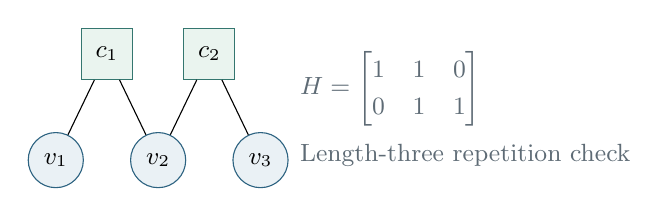
\begin{tikzpicture}[
  var/.style={circle,draw=blue,fill=paleBlue,minimum size=7mm},
  chk/.style={rectangle,draw=teal,fill=paleGreen,minimum size=6.5mm},
  every node/.style={font=\small}
]
  \node[var] (v1) at (0,0) {$v_1$};
  \node[var] (v2) at (1.3,0) {$v_2$};
  \node[var] (v3) at (2.6,0) {$v_3$};
  \node[chk] (c1) at (0.65,1.35) {$c_1$};
  \node[chk] (c2) at (1.95,1.35) {$c_2$};
  \draw (c1)--(v1) (c1)--(v2) (c2)--(v2) (c2)--(v3);
  \node[align=left,text=muted] at (5.2,0.65) {$H=\begin{bmatrix}1&1&0\\0&1&1\end{bmatrix}$\\[2mm]
  Length-three repetition check};
\end{tikzpicture}
\end{center}

For this matrix, the kernel contains $000$ and $111$, so the classical code has parameters
$[3,1,3]$. This small check matrix will be used twice in the project fixture.

\begin{keyidea}
The matrix view is ideal for algebra and validation. The Tanner-graph view is ideal for sparse
computation and human explanation. The explorer should let a user move between both without
changing the underlying experiment state.
\end{keyidea}

\section{Quantum stabilizer and CSS foundations}

\subsection{Pauli errors as binary data}

Ignoring global phase, an $n$-qubit Pauli operator can be represented by two binary vectors:
\begin{equation}
  E \longleftrightarrow (e_X\mid e_Z)\in\F^{2n}.
\end{equation}
At qubit $j$, the pair $(e_{X,j},e_{Z,j})$ means
\begin{center}
\begin{tabular}{c c c}
\toprule
$e_{X,j}$ & $e_{Z,j}$ & Pauli \\
\midrule
0 & 0 & $I$ \\
1 & 0 & $X$ \\
0 & 1 & $Z$ \\
1 & 1 & $Y$ up to phase \\
\bottomrule
\end{tabular}
\end{center}

Two Paulis $(x\mid z)$ and $(x'\mid z')$ commute exactly when their symplectic product vanishes:
\begin{equation}
  xz'^{\mathsf T}+zx'^{\mathsf T}=0\pmod 2.
\end{equation}

\subsection{Stabilizer codes}

A stabilizer code is the joint $+1$ eigenspace of an abelian subgroup $\mathcal S$ of the Pauli
group that excludes $-I$. If there are $r$ independent stabilizer generators on $n$ qubits, the
codespace encodes $k=n-r$ logical qubits.

An error has a nonzero syndrome when it anticommutes with one or more measured stabilizer
generators. Stabilizers themselves act trivially on the logical state. This creates the central
feature of quantum decoding: many physically different errors are logically equivalent.

\subsection{CSS codes}

A CSS code separates stabilizer generators into $X$-type and $Z$-type checks. Let
\begin{equation}
  H_X\in\F^{m_X\times n},\qquad H_Z\in\F^{m_Z\times n}.
\end{equation}
Rows of $H_X$ locate $X$ operators in $X$-type stabilizers; rows of $H_Z$ locate $Z$ operators in
$Z$-type stabilizers. Commutation is exactly the matrix condition
\begin{equation}
  H_XH_Z^{\mathsf T}=0.
  \label{eq:css-orthogonality}
\end{equation}
The number of logical qubits is
\begin{equation}
  k=n-\rank(H_X)-\rank(H_Z).
\end{equation}

For an error $(e_X\mid e_Z)$, the check-type convention gives
\begin{equation}
  s_X=H_Xe_Z^{\mathsf T},\qquad s_Z=H_Ze_X^{\mathsf T}.
  \label{eq:css-syndrome}
\end{equation}
$X$ checks detect the $Z$ component, while $Z$ checks detect the $X$ component. A $Y$ error has
both components and can activate both syndromes.

\begin{warningbox}[Syndrome naming convention]
Some software names $s_X$ after the error component being decoded, not the check type being
measured. Both conventions exist. Every API, plot, and decoder trace must state its convention.
The equations in this guide name a syndrome after its check type.
\end{warningbox}

\subsection{Logical operators and distance}

An $X$-type operator commutes with all $Z$ checks when its support vector lies in $\ker H_Z$.
It is a trivial stabilizer when it lies in $\rowspan(H_X)$. Therefore
\begin{align}
  d_X &= \min\{\wt(x):x\in\ker H_Z\setminus\rowspan(H_X)\},\\
  d_Z &= \min\{\wt(z):z\in\ker H_X\setminus\rowspan(H_Z)\},\\
  d &= \min(d_X,d_Z).
\end{align}
A code with distance $d$ corrects every adversarial error of weight at most
$\lfloor(d-1)/2\rfloor$. Under a stochastic noise model, larger errors may also be corrected; the
distance guarantee is a worst-case statement.

\subsection{What makes a code qLDPC?}

A CSS family is qLDPC when $H_X$ and $H_Z$ remain sparse as $n$ grows: stabilizer weights and the
number of stabilizers touching each qubit remain bounded. The notation $[[n,k,d]]$ records block
length, logical dimension, and distance, but it does not record check weight, graph degree,
connectivity, decoder complexity, or measurement-circuit cost. Those must be reported separately.

\section{The hypergraph-product construction}

\subsection{Inputs and qubit sectors}

Take two classical binary parity-check matrices
\begin{equation}
  H_1\in\F^{r_1\times n_1},\qquad H_2\in\F^{r_2\times n_2}.
\end{equation}
The HGP construction creates two sectors of physical qubits:
\begin{equation}
  Q_{VV}=V_1\times V_2,\qquad Q_{CC}=C_1\times C_2.
\end{equation}
Their sizes are $n_1n_2$ and $r_1r_2$, so the total block length is
\begin{equation}
  n=n_1n_2+r_1r_2.
\end{equation}

\begin{center}
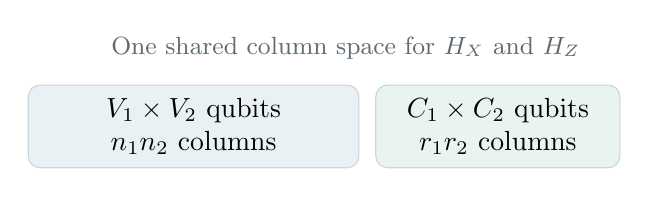
\begin{tikzpicture}[
  block/.style={draw=line,rounded corners=1.5mm,minimum height=1.05cm,align=center},
  label/.style={font=\small,text=muted}
]
  \node[block,fill=paleBlue,minimum width=4.2cm] (vv) {$V_1\times V_2$ qubits\\$n_1n_2$ columns};
  \node[block,fill=paleGreen,minimum width=3.1cm,right=2mm of vv] (cc) {$C_1\times C_2$ qubits\\$r_1r_2$ columns};
  \node[label,above=2mm of $(vv.north)!0.5!(cc.north)$] {One shared column space for $H_X$ and $H_Z$};
\end{tikzpicture}
\end{center}

\subsection{Check matrices}

With a consistent Kronecker-product ordering, define
\begin{align}
  H_X &= \left[H_1\otimes I_{n_2}\ \middle|\ I_{r_1}\otimes H_2^{\mathsf T}\right],
  \label{eq:hgp-hx}\\
  H_Z &= \left[I_{n_1}\otimes H_2\ \middle|\ H_1^{\mathsf T}\otimes I_{r_2}\right].
  \label{eq:hgp-hz}
\end{align}
The dimensions are
\begin{align}
  H_X &: (r_1n_2)\times(n_1n_2+r_1r_2),\\
  H_Z &: (n_1r_2)\times(n_1n_2+r_1r_2).
\end{align}

\subsection{Why the checks commute}

Multiplying the two block matrices gives
\begin{align}
H_XH_Z^{\mathsf T}
&=(H_1\otimes I_{n_2})(I_{n_1}\otimes H_2^{\mathsf T})
 +(I_{r_1}\otimes H_2^{\mathsf T})(H_1\otimes I_{r_2})\\
&=H_1\otimes H_2^{\mathsf T}+H_1\otimes H_2^{\mathsf T}\\
&=0\pmod 2.
\end{align}
The two equal terms cancel because arithmetic is binary. This is the algebraic heart of the HGP
construction: commutation is built in rather than checked by trial and error.

\subsection{Dimension}

Define
\begin{equation}
  k_i=n_i-\rank(H_i),\qquad k_i^{\mathsf T}=r_i-\rank(H_i).
\end{equation}
Then the HGP code dimension is
\begin{equation}
  k=k_1k_2+k_1^{\mathsf T}k_2^{\mathsf T}.
  \label{eq:hgp-k}
\end{equation}
The transpose-code terms matter when the input checks have dependent rows.

\subsection{Distance intuition}

Logical operators descend from codewords and transpose-code codewords of the classical inputs.
Under the usual nontriviality conditions, the HGP distance is controlled by the smallest relevant
input distance. Families built from suitable classical LDPC codes can achieve constant rate and
distance proportional to $\sqrt n$ \cite{tillich-zemor}. The exact distance of a finite instance
should be computed or bounded rather than inferred only from asymptotic statements.

\begin{keyidea}[The construction in one sentence]
The HGP takes two sparse classical constraint systems, creates qubits from variable-variable and
check-check pairs, and uses Kronecker products to produce sparse commuting quantum checks.
\end{keyidea}

\section{Worked example: the project fixture \texorpdfstring{$[[13,1,3]]$}{[[13,1,3]]}}

\subsection{Classical input}

Use the length-three repetition check for both inputs:
\begin{equation}
  H_1=H_2=H=\begin{bmatrix}
  1&1&0\\
  0&1&1
  \end{bmatrix}.
\end{equation}
Here $n_1=n_2=3$, $r_1=r_2=2$, $\rank(H)=2$, $k_1=k_2=1$, and
$k_1^{\mathsf T}=k_2^{\mathsf T}=0$.

\subsection{Derived parameters}

The HGP formulas immediately give
\begin{align}
  n &= 3\cdot3+2\cdot2=13,\\
  k &= 1\cdot1+0\cdot0=1.
\end{align}
The construction produces six $X$-check rows and six $Z$-check rows. For this fixture both check
matrices have rank six, so $k=13-6-6=1$. Exact enumeration gives $d_X=d_Z=3$, hence
\begin{equation}
  [[n,k,d]]=[[13,1,3]].
\end{equation}

\begin{center}
\begin{tabularx}{0.88\textwidth}{>{\bfseries\color{navy}}l X r}
\toprule
Property & Meaning & Value \\
\midrule
Physical qubits $n$ & Columns shared by $H_X,H_Z$ & 13 \\
Logical qubits $k$ & Protected degrees of freedom & 1 \\
Distance $d$ & Minimum nontrivial logical Pauli weight & 3 \\
$X$ checks & Rows of $H_X$ & 6 \\
$Z$ checks & Rows of $H_Z$ & 6 \\
Check weights & Number of qubits per generator & 3 or 4 \\
Guaranteed correction & All errors through weight $\lfloor(d-1)/2\rfloor$ & 1 \\
\bottomrule
\end{tabularx}
\end{center}

\subsection{Why this is a useful teaching code}

\begin{itemize}
  \item It is small enough to show every qubit, check, and nonzero syndrome.
  \item Its construction still exercises the real HGP algebra and two qubit sectors.
  \item Exact distance and exhaustive decoding are feasible, providing an oracle for tests.
  \item Weight-three logical operators make success and failure examples easy to construct.
  \item The code is not presented as a performance benchmark for large-scale fault tolerance.
\end{itemize}

\begin{projectbox}
The Configure stage already exposes this fixture and its calculated validation evidence. Inject,
Observe, and Decode should consume the same immutable code identifier and matrix ordering. A user
selection such as ``qubit 7 receives $Y$'' is meaningful only if all stages share that ordering.
\end{projectbox}

\section{Noise models and error injection}

\subsection{Code-capacity noise}

The first project model assumes perfect stabilizer measurements and applies noise only to data
qubits. This is the code-capacity setting. For independent depolarizing noise,
\begin{equation}
  \Pr(I)=1-p,\qquad \Pr(X)=\Pr(Y)=\Pr(Z)=\frac{p}{3}.
  \label{eq:depolarizing}
\end{equation}
Alternative independent channels can assign different probabilities $p_X,p_Y,p_Z$ as long as they
sum to at most one.

The model is intentionally simple. It isolates code and decoder behavior from measurement-circuit
design, repeated rounds, leakage, and time correlations.

\subsection{Manual injection}

Manual mode should let a learner choose qubits and Pauli types directly. The internal state is the
pair $(e_X,e_Z)$. Adding another Pauli on the same qubit uses Pauli multiplication up to phase,
which becomes XOR in the binary representation. For example,
\begin{equation}
  X\cdot Z\sim Y,\qquad (1,0)+(0,1)=(1,1).
\end{equation}
The interface may either replace the selected Pauli or explicitly compose it, but the rule must be
visible and deterministic.

\subsection{Seeded stochastic injection}

A reproducible run stores at least
\begin{equation}
  (\text{code version},\text{noise model},p,\text{seed},\text{generator version}).
\end{equation}
The seed alone is insufficient if sampling order or pseudorandom generator behavior later changes.
The generated error should be stored as part of the run record so that a historical result remains
inspectable.

\subsection{Later noise-model layers}

\begin{longtable}{>{\bfseries}p{0.22\textwidth} p{0.33\textwidth} p{0.36\textwidth}}
\toprule
Model & Adds & Why it is harder \\
\midrule
\endfirsthead
\toprule
Model & Adds & Why it is harder \\
\midrule
\endhead
Code capacity & Data-qubit Pauli errors; perfect measurements & One syndrome snapshot; suitable for the first implementation \\
Phenomenological & Data errors plus noisy syndrome bits across rounds & Decoder must use space-time information \\
Circuit level & Faults on gates, preparation, idling, and measurement & A single fault can propagate to correlated data and measurement errors \\
Biased or correlated & Unequal Pauli rates or multi-qubit events & Independent binary decoding may discard useful correlations \\
Erasure & Error locations are known, values may be unknown & Different likelihood model and often easier combinatorics \\
\bottomrule
\end{longtable}

\begin{warningbox}
A threshold is never just a property of a check matrix. It belongs to a combination of code family,
decoder, noise model, syndrome-extraction model, and scaling experiment.
\end{warningbox}

\section{Syndromes: what the system observes}

\subsection{Calculating the two syndrome channels}

Given $(e_X,e_Z)$, calculate the syndromes using Equation~\eqref{eq:css-syndrome}. Each syndrome bit
is the parity of error components adjacent to that check. In graph language, a check is activated
when it has odd overlap with the anticommuting component of the error.

\begin{center}
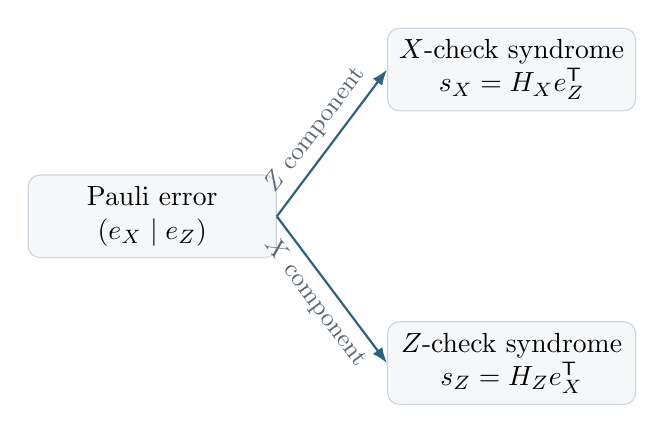
\begin{tikzpicture}[
  box/.style={draw=line,rounded corners=1.5mm,minimum width=3.15cm,minimum height=1.05cm,align=center,fill=paper},
  arrow/.style={-{Latex[length=2mm]},thick,draw=blue},
  lab/.style={font=\small,text=muted,align=center}
]
  \node[box] (err) {Pauli error\\$(e_X\mid e_Z)$};
  \node[box,above right=8mm and 14mm of err] (sx) {$X$-check syndrome\\$s_X=H_Xe_Z^{\mathsf T}$};
  \node[box,below right=8mm and 14mm of err] (sz) {$Z$-check syndrome\\$s_Z=H_Ze_X^{\mathsf T}$};
  \draw[arrow] (err.east) -- node[lab,above,sloped] {$Z$ component} (sx.west);
  \draw[arrow] (err.east) -- node[lab,below,sloped] {$X$ component} (sz.west);
\end{tikzpicture}
\end{center}

\subsection{What a syndrome does and does not reveal}

The syndrome reveals an equivalence class of candidate errors. If $e$ and $e'$ differ by an element
of the kernel of the relevant check matrix, then they have the same syndrome. In a quantum code,
same-syndrome candidates can differ by:

\begin{itemize}
  \item a stabilizer, in which case they act identically on logical information; or
  \item a logical operator, in which case choosing the wrong class causes logical failure.
\end{itemize}

This is why syndrome matching is necessary but not sufficient for successful decoding.

\subsection{Observe-stage representations}

The project should present the same syndrome through linked views:

\begin{itemize}
  \item a compact binary vector for exactness and export;
  \item a check list with satisfied and violated constraints;
  \item a Tanner-graph view that highlights local neighborhoods; and
  \item a matrix view that shows the parity calculation for a selected check.
\end{itemize}

Selecting a check in one view should highlight the same check and neighboring qubits in the others.
This supports recognition, causal reasoning, and debugging without adding scientific state.

\section{The quantum decoding problem}

\subsection{Decoder input and output}

For one CSS component, a decoder receives a check matrix $H$, syndrome $s$, and a noise prior. It
returns a candidate correction $\hat e$ satisfying
\begin{equation}
  H\hat e^{\mathsf T}=s.
  \label{eq:syndrome-consistency}
\end{equation}
For the full CSS code, corrections $(\hat e_X,\hat e_Z)$ are produced from the two syndrome
channels with consistent conventions.

\subsection{The real success condition}

Let $E$ be the actual error and $R$ the proposed recovery. Decoding succeeds when
\begin{equation}
  RE\in\mathcal S,
  \label{eq:logical-success}
\end{equation}
up to an irrelevant phase. In binary addition, the residual error $e+\hat e$ must be a stabilizer.
It need not be the zero vector. This distinction is degeneracy.

\begin{center}
\begin{tabularx}{\textwidth}{>{\bfseries}p{0.2\textwidth} X X}
\toprule
Outcome & Syndrome test & Logical test \\
\midrule
Invalid correction & $H\hat e^{\mathsf T}\ne s$ & Decoder failed to return a feasible correction \\
Successful recovery & $H\hat e^{\mathsf T}=s$ & Residual is a stabilizer \\
Logical failure & $H\hat e^{\mathsf T}=s$ & Residual is a nontrivial logical operator \\
\bottomrule
\end{tabularx}
\end{center}

\subsection{Maximum-likelihood objectives}

A nondegenerate decoder might choose the most likely physical error:
\begin{equation}
  \hat e_{\mathrm{physical}}=\arg\max_{e:He^{\mathsf T}=s}\Pr(e\mid s).
\end{equation}
A degenerate maximum-likelihood decoder instead chooses the most likely logical equivalence class:
\begin{equation}
  \hat{\mathcal C}=\arg\max_{\mathcal C}\sum_{e\in\mathcal C}\Pr(e\mid s).
\end{equation}
The second objective is the quantum-correct one, but it is generally more difficult. Practical
decoders approximate it in different ways.

\subsection{Two independent binary decoders or one correlated decoder?}

For independent $X$ and $Z$ noise, a CSS decoder can treat the components separately. Under
depolarizing noise, a $Y$ error couples both components, so separate decoding discards correlation.
The first project implementation can use separate channels because it makes every step legible. A
later correlated decoder should be evaluated against the same run records.

\section{Decoder families relevant to HGP qLDPC codes}

\subsection{Exact lookup or exhaustive decoding}

For the $[[13,1,3]]$ fixture, enumerate errors or syndrome-consistent candidates and classify their
logical cosets. Exact decoding is exponentially expensive in $n$, but it provides:

\begin{itemize}
  \item an interpretable first decoder;
  \item a correctness oracle for optimized decoders;
  \item exact examples of degeneracy and tie breaking; and
  \item deterministic traces suitable for teaching.
\end{itemize}

A useful baseline selects a minimum-weight candidate, applies a deterministic lexicographic tie
break, verifies Equation~\eqref{eq:syndrome-consistency}, and reports the residual logical class.

\subsection{Belief propagation}

Belief propagation (BP) passes probabilistic messages along the Tanner graph. For a binary
symmetric channel with crossover probability $p$, the prior log-likelihood ratio is
\begin{equation}
  L_j^{(0)}=\log\frac{1-p}{p}.
\end{equation}
In sum-product BP, a check-to-variable update has the form
\begin{equation}
  L_{a\rightarrow j}=2\operatorname{atanh}\left(
  (-1)^{s_a}\prod_{j'\in N(a)\setminus j}\tanh\frac{L_{j'\rightarrow a}}{2}
  \right),
\end{equation}
and a variable-to-check update combines the prior with other incoming checks:
\begin{equation}
  L_{j\rightarrow a}=L_j^{(0)}+\sum_{b\in N(j)\setminus a}L_{b\rightarrow j}.
\end{equation}
On a tree, BP gives exact marginals. qLDPC Tanner graphs contain cycles, and quantum degeneracy can
create symmetric or split beliefs. BP may oscillate, converge to an inconsistent hard decision, or
settle on a poor logical class.

\subsection{BP with ordered-statistics decoding}

BP+OSD uses BP to estimate bit reliabilities, then invokes linear-algebraic post-processing when a
reliable syndrome-consistent answer is needed. It has demonstrated broad utility for HGP qLDPC
codes \cite{roffe-bposd}.

At a high level:
\begin{enumerate}
  \item run BP for a fixed number of iterations or until a stopping rule;
  \item sort columns by reliability;
  \item select an information or pivot structure through elimination;
  \item construct a syndrome-consistent baseline candidate; and
  \item test low-order flips among selected unreliable positions, retaining the best metric.
\end{enumerate}

OSD order controls a performance-complexity tradeoff. Order zero tests the elimination-derived
candidate. Higher orders enumerate more perturbations. The decoder trace should record BP
iterations, final reliabilities, permutation, OSD order, candidates tested, and selection metric.

\subsection{Small-set-flip}

Small-set-flip is designed for quantum expander codes, a structured subclass of HGP codes. It
repeatedly chooses a small subset supported within a stabilizer neighborhood whose flip reduces
the syndrome sufficiently. Under expansion assumptions it has strong provable correction and
runtime guarantees \cite{leverrier-expander}.

The $[[13,1,3]]$ teaching fixture should not be described as satisfying those asymptotic expansion
guarantees without checking the hypotheses. The algorithm remains valuable conceptually because
its progress measure is visible: each accepted local flip changes the residual syndrome.

\subsection{Other useful directions}

\begin{itemize}
  \item \textbf{BP with guided decimation:} progressively fixes highly reliable variables to break
  symmetry and encourage convergence \cite{yao-bpgd}.
  \item \textbf{Localized statistics decoding:} performs inversion-based post-processing on local
  clusters rather than one global system.
  \item \textbf{Generalized union-find:} grows and merges syndrome regions; extensions have been
  studied for broader qLDPC families \cite{delfosse-union-find}.
  \item \textbf{Integer or tensor-network methods:} can provide strong baselines on limited sizes,
  usually at greater computational cost.
\end{itemize}

\begin{keyidea}[Recommended implementation sequence]
Start with exact minimum-weight lookup for the small fixture, because it makes correctness
observable. Add BP with a complete message trace. Then add OSD post-processing and compare it to
the exact oracle. This sequence separates implementation errors from algorithmic limitations.
\end{keyidea}

\section{A detailed BP+OSD decoding trace}

This section defines the information the Decode stage should expose for one binary component.

\subsection{Inputs}

\begin{itemize}
  \item check matrix $H$ and its stable row and column ordering;
  \item observed syndrome $s$;
  \item channel prior $p$ or per-qubit priors;
  \item BP update rule, schedule, damping factor, and maximum iterations;
  \item OSD method, order, and candidate metric; and
  \item deterministic tie-breaking policy.
\end{itemize}

\subsection{BP phase}

For each iteration, retain summary values rather than every transient UI animation:

\begin{enumerate}
  \item compute check-to-variable messages from the previous variable messages;
  \item compute variable-to-check messages and posterior beliefs;
  \item form a hard decision $\hat e^{(t)}$;
  \item compute the predicted syndrome $H\hat e^{(t)\mathsf T}$;
  \item record whether the target syndrome is satisfied; and
  \item stop according to the declared rule.
\end{enumerate}

Useful diagnostics include maximum message change, number of unsatisfied checks, hard-decision
weight, and whether a state repeated. Message clipping and damping must be reported because they
can materially change convergence.

\subsection{OSD phase}

OSD consumes BP reliabilities, but its output must still be verified independently. The trace
should show:

\begin{itemize}
  \item reliability-ranked qubits;
  \item the column permutation used for elimination;
  \item pivot and free positions;
  \item the baseline candidate and each tested perturbation class;
  \item the candidate cost under the noise model; and
  \item the final syndrome-consistency result.
\end{itemize}

\subsection{Outcome classification}

After combining the $X$ and $Z$ corrections, compute the residual $E+R$. Report three separate
facts:

\begin{enumerate}
  \item \textbf{feasibility:} did the correction reproduce the observed syndrome?
  \item \textbf{logical result:} is the residual a stabilizer or a nontrivial logical operator?
  \item \textbf{effort:} how many iterations, candidates, and units of time were used?
\end{enumerate}

The user should never have to infer logical success from a green ``converged'' label. Convergence
and correctness are different.

\section{Project architecture and data contracts}

\subsection{Scientific state model}

A run should be a versioned record rather than a loose collection of interface fields. A compact
conceptual schema is:

\begin{tcolorbox}[colback=paper,colframe=line,fontupper=\small\ttfamily]
run = \{\par
\quad code: \{id, version, Hx, Hz, parameters, ordering\},\par
\quad model: \{noise family, probability, measurement assumptions\},\par
\quad injection: \{mode, seed, Pauli error\},\par
\quad observation: \{sx, sz, convention\},\par
\quad decoding: \{decoder, settings, correction, trace\},\par
\quad outcome: \{syndrome consistent, logical class, metrics\}\par
\}
\end{tcolorbox}

Derived values should be recomputable from earlier state. For example, the Observe stage should not
accept an arbitrary syndrome as if it came from the stored error unless the run is explicitly in a
manual-syndrome mode.

\subsection{Stage contracts}

\begin{longtable}{@{}>{\bfseries}p{0.14\textwidth} p{0.28\textwidth} p{0.28\textwidth} p{0.21\textwidth}@{}}
\toprule
Stage & Inputs & Outputs & Core invariant \\
\midrule
\endfirsthead
\toprule
Stage & Inputs & Outputs & Core invariant \\
\midrule
\endhead
Configure & Code identifier, noise choice, parameters, seed & Confirmed immutable configuration & Code evidence and assumptions are valid \\
Inject & Confirmed configuration & Explicit $(e_X,e_Z)$ and Pauli labels & Binary and Pauli views agree \\
Observe & Code matrices and error & $(s_X,s_Z)$ plus check states & Syndromes equal matrix products \\
Decode & Matrices, syndrome, priors, decoder settings & Correction, trace, residual class & Output is independently verified \\
\bottomrule
\end{longtable}

\subsection{API responsibilities}

The backend should own scientific calculations and validation. The frontend should own interaction,
linked views, and presentation. This division avoids two independent implementations silently
disagreeing. Suggested service boundaries are:

\begin{itemize}
  \item \code{GET /api/codes}: list verified code fixtures and summaries;
  \item \code{GET /api/codes/\{id\}}: retrieve matrices, parameters, conventions, and evidence;
  \item \code{POST /api/injections}: validate or generate a reproducible Pauli error;
  \item \code{POST /api/syndromes}: calculate syndromes and per-check explanations;
  \item \code{POST /api/decodings}: run a named decoder with explicit settings; and
  \item \code{GET /api/runs/\{id\}}: retrieve a complete reproducible record when persistence is added.
\end{itemize}

These are design targets, not claims that every endpoint is already implemented.

\section{Human-centered scientific interaction}

The HCI objective is not to simplify away the mathematics. It is to control complexity while
preserving causal and scientific meaning.

\subsection{Interaction principles}

\begin{itemize}
  \item \textbf{Progressive disclosure:} show the decision first, then matrices, traces, and proofs
  on demand.
  \item \textbf{Visibility of state:} distinguish draft, confirmed, generated, observed, decoding,
  and verified states.
  \item \textbf{Recognition over recall:} label Pauli types, check conventions, and parameter
  meanings near the control that uses them.
  \item \textbf{Error prevention:} constrain probabilities, seeds, qubit indices, and incompatible
  settings before execution.
  \item \textbf{Reversibility:} allow edits by returning to the earliest affected stage and clearly
  invalidating downstream results.
  \item \textbf{Multiple coordinated representations:} link matrix, graph, vector, and textual
  explanations to one canonical state.
  \item \textbf{Honest uncertainty:} attach confidence intervals and sample counts to empirical
  performance claims.
\end{itemize}

\subsection{Visual semantics}

Color should be redundant, not exclusive. An activated check needs a symbol and text label in
addition to color. $X$, $Y$, and $Z$ should have stable encodings across all stages. Focus order,
keyboard operation, sufficient contrast, and screen-reader labels are part of scientific usability:
a user who cannot access a graph must still access the same check and syndrome data.

\subsection{Details on demand}

A well-layered Decode result might show:

\begin{enumerate}
  \item first: logical success or failure, correction weight, and runtime;
  \item next: syndrome consistency and residual class;
  \item then: iteration-level decoder diagnostics; and
  \item finally: raw messages, permutations, candidate lists, and exported run data.
\end{enumerate}

This ordering serves both a learner asking ``what happened?'' and a researcher asking ``why?''
without creating separate products.

\section{Experimental methodology}

\subsection{Single-run diagnostics}

One run is useful for explanation and debugging. Record:

\begin{itemize}
  \item actual error weight and Pauli composition;
  \item syndrome weights $\wt(s_X)$ and $\wt(s_Z)$;
  \item correction weight;
  \item residual stabilizer or logical class;
  \item decoder convergence, iterations, and candidate count; and
  \item wall-clock time measured under a declared environment.
\end{itemize}

\subsection{Monte Carlo experiments}

At each physical error rate $p$, run $N$ independent trials and count $F$ logical failures. The
estimated logical error rate is
\begin{equation}
  \widehat p_L=\frac{F}{N}.
\end{equation}
Always report $N$ and an interval estimate. When $F$ is small, the naive normal interval is poor;
a Wilson or exact binomial interval is more appropriate.

To compare decoders fairly, reuse the same sampled errors when possible. Paired trials reduce noise
in the comparison and make disagreements directly inspectable.

\subsection{Threshold studies}

A threshold study requires a family of increasing code sizes and curves of logical error rate
versus physical error rate under fixed decoder and noise definitions. The small $[[13,1,3]]$
fixture alone cannot establish a threshold. It can validate the experiment pipeline before larger
HGP instances are added.

\subsection{Metrics beyond logical error rate}

\begin{itemize}
  \item throughput and latency distributions, not only averages;
  \item memory usage and message count;
  \item fraction of outputs that are syndrome inconsistent;
  \item convergence rate and iteration distribution;
  \item performance by error weight or syndrome weight;
  \item failure-mode taxonomy: nonconvergence, wrong logical class, timeout, or invalid result; and
  \item sensitivity to decoder hyperparameters and seed.
\end{itemize}

\section{Verification and testing strategy}

\subsection{Code-construction invariants}

Every registered code should satisfy automated checks for:

\begin{enumerate}
  \item binary entries and compatible dimensions;
  \item CSS orthogonality $H_XH_Z^{\mathsf T}=0$;
  \item claimed ranks and $k=n-r_X-r_Z$;
  \item bounded check and qubit degrees for the intended family;
  \item exact or independently justified distance for small fixtures; and
  \item stable row and column ordering with a version identifier.
\end{enumerate}

\subsection{Stage-level properties}

\begin{center}
\begin{tabularx}{\textwidth}{>{\bfseries}p{0.18\textwidth} X}
\toprule
Component & Property test \\
\midrule
Pauli conversion & Pauli $\leftrightarrow(e_X,e_Z)$ round trip is exact \\
Injection & Same code, model, probability, generator version, and seed reproduce the same error \\
Syndrome & Per-check parity view equals the matrix product \\
Correction & Every accepted correction reproduces the input syndrome \\
Logical classifier & Stabilizers classify as success; known logicals classify as failure \\
Exact decoder & Corrects every error of weight at most one for the $[[13,1,3]]$ fixture \\
BP+OSD & Matches the exact oracle on a regression corpus where expected behavior is fixed \\
Serialization & Exported and reloaded runs preserve all scientific fields \\
\bottomrule
\end{tabularx}
\end{center}

\subsection{Independent verification}

Whenever practical, calculate important claims by two paths. For example, obtain the fixture
distance by exhaustive logical search and separately verify that all weight-one errors are
correctable while a weight-three logical exists. A decoder should not be responsible for grading
its own output; residual classification belongs to a separate verifier.

\begin{projectbox}[Definition of done for a scientific slice]
A stage is complete when its state contract, calculations, UI, accessibility, deterministic
examples, automated tests, and failure messages agree. A visually complete screen without a
verified scientific transition is not complete.
\end{projectbox}

\section{Implementation roadmap}

\subsection{Current foundation: Configure}

\begin{itemize}
  \item versioned qLDPC fixture registry;
  \item verified $[[13,1,3]]$ HGP construction and evidence;
  \item manual or seeded code-capacity setup; and
  \item confirmed configuration state shared with later stages.
\end{itemize}

\subsection{Next slice: Inject}

\begin{itemize}
  \item canonical Pauli-error representation and validation;
  \item interactive 13-qubit selection with $I,X,Y,Z$ states;
  \item seeded independent-noise generation;
  \item error summary, weight, and reproducibility metadata; and
  \item invalidation of downstream results when the error changes.
\end{itemize}

\subsection{Then: Observe}

\begin{itemize}
  \item backend syndrome calculation from stored matrices and error vectors;
  \item separated $X$-check and $Z$-check channels with explicit naming;
  \item linked check-list, matrix, and Tanner-graph views;
  \item selected-check parity explanation; and
  \item syndrome invariants and export.
\end{itemize}

\subsection{Then: Decode}

\begin{itemize}
  \item exact minimum-weight decoder for the teaching fixture;
  \item independent correction verifier and logical-outcome classifier;
  \item stepwise trace and counterexamples illustrating degeneracy;
  \item BP implementation with configurable schedule, damping, and stopping; and
  \item OSD post-processing with reliability and candidate inspection.
\end{itemize}

\subsection{Research extensions}

After the single-run workflow is correct, add larger HGP families, batch experiments, confidence
intervals, decoder comparisons, and performance profiling. Phenomenological or circuit-level noise
should be a later architectural extension because it changes the data model from one syndrome
snapshot to a history of noisy measurements.

\section{Study questions and practical exercises}

\subsection{Concept checks}

\begin{enumerate}
  \item Why does $H_XH_Z^{\mathsf T}=0$ encode commutation?
  \item Why can two different errors with the same syndrome lead to different logical outcomes?
  \item What information is missing from the notation $[[n,k,d]]$?
  \item Why does a $Y$ error contribute to both binary error components?
  \item Why is decoder convergence not equivalent to decoding success?
  \item Why can the $[[13,1,3]]$ code validate a pipeline but not establish a threshold?
\end{enumerate}

\subsection{Matrix exercises}

\begin{enumerate}
  \item Verify that the length-three repetition check has rank two and kernel
  $\{000,111\}$.
  \item Use Equations~\eqref{eq:hgp-hx}--\eqref{eq:hgp-hz} to derive the dimensions of the two
  project check matrices.
  \item Pick one single-qubit $X$ error and calculate its $Z$-check syndrome from the matrix in
  Appendix~\ref{app:matrices}.
  \item Pick one single-qubit $Y$ error and calculate both syndrome channels.
  \item Find two distinct syndrome-consistent candidates and determine whether their difference is
  a stabilizer or logical operator.
\end{enumerate}

\subsection{Implementation exercises}

\begin{enumerate}
  \item Write a property test that every manual Pauli selection round-trips through the binary
  representation.
  \item Create a deterministic lookup table from syndrome to minimum-weight correction for one CSS
  component.
  \item Construct a failing example in which a syndrome-consistent correction leaves a logical
  residual.
  \item Compare BP hard decisions before and after damping on one cyclic Tanner graph.
  \item Design an export record that is sufficient to replay a historical run after the codebase
  changes.
\end{enumerate}

\clearpage
\appendix

\section{Notation and glossary}

\begin{longtable}{>{\bfseries}p{0.20\textwidth} p{0.70\textwidth}}
\toprule
Term or symbol & Meaning \\
\midrule
\endfirsthead
\toprule
Term or symbol & Meaning \\
\midrule
\endhead
$\F$ & Binary field; addition and multiplication are modulo two \\
$H$ & Classical parity-check matrix \\
$H_X,H_Z$ & Binary support matrices for CSS $X$- and $Z$-type stabilizer generators \\
$[[n,k,d]]$ & Quantum block length, number of logical qubits, and code distance \\
Syndrome & Outcomes identifying which stabilizer checks anticommute with an error \\
Stabilizer & Pauli operator that acts trivially on every encoded state \\
Logical operator & Pauli in the stabilizer normalizer but not in the stabilizer group \\
Degeneracy & Different physical errors or corrections that have the same logical action \\
Tanner graph & Bipartite graph connecting check nodes to variable or qubit nodes \\
qLDPC & Quantum code family with sparse, bounded-weight parity checks \\
HGP & Hypergraph-product construction from two classical parity-check matrices \\
Code-capacity noise & Data-qubit noise with perfect stabilizer measurement \\
BP & Belief propagation message passing on a factor or Tanner graph \\
OSD & Ordered-statistics post-processing using reliabilities and elimination \\
Residual & Product, or binary sum, of actual error and proposed recovery \\
Logical failure rate & Probability that the residual contains a nontrivial logical action \\
\bottomrule
\end{longtable}

\begin{landscape}
\thispagestyle{empty}
\section{Explicit matrices for the \texorpdfstring{$[[13,1,3]]$}{[[13,1,3]]} fixture}
\label{app:matrices}

The following matrices use the project construction's current Kronecker ordering. Columns 1--9
belong to the $V_1\times V_2$ sector and columns 10--13 belong to the $C_1\times C_2$ sector.

\begin{equation}
\scriptsize
H_X=\left[
\begin{array}{ccccccccc|cccc}
1&0&0&1&0&0&0&0&0&1&0&0&0\\
0&1&0&0&1&0&0&0&0&1&1&0&0\\
0&0&1&0&0&1&0&0&0&0&1&0&0\\
0&0&0&1&0&0&1&0&0&0&0&1&0\\
0&0&0&0&1&0&0&1&0&0&0&1&1\\
0&0&0&0&0&1&0&0&1&0&0&0&1
\end{array}
\right].
\end{equation}

\begin{equation}
\scriptsize
H_Z=\left[
\begin{array}{ccccccccc|cccc}
1&1&0&0&0&0&0&0&0&1&0&0&0\\
0&1&1&0&0&0&0&0&0&0&1&0&0\\
0&0&0&1&1&0&0&0&0&1&0&1&0\\
0&0&0&0&1&1&0&0&0&0&1&0&1\\
0&0&0&0&0&0&1&1&0&0&0&1&0\\
0&0&0&0&0&0&0&1&1&0&0&0&1
\end{array}
\right].
\end{equation}

The row weights of $H_X$ are $(3,4,3,3,4,3)$ and those of $H_Z$ are
$(3,3,4,4,3,3)$. Direct multiplication verifies $H_XH_Z^{\mathsf T}=0$.
\end{landscape}

\section{Decoder comparison worksheet}

\begin{longtable}{>{\bfseries}p{0.18\textwidth} p{0.20\textwidth} p{0.20\textwidth} p{0.30\textwidth}}
\toprule
Decoder & Main strength & Main limitation & Evidence to expose \\
\midrule
\endfirsthead
\toprule
Decoder & Main strength & Main limitation & Evidence to expose \\
\midrule
\endhead
Exact lookup & Ground-truth behavior on tiny codes & Exponential scaling & Candidates, tie break, residual class \\
BP & Sparse and fast per iteration & Cycles and degeneracy can prevent useful convergence & Messages, beliefs, unsatisfied checks \\
BP+OSD & Robust syndrome-consistent post-processing & Elimination and candidate cost grow with order & Reliability ordering, pivots, candidates \\
Small-set-flip & Local steps and strong expander-code theory & Guarantees require expansion hypotheses & Selected flips and syndrome reduction \\
Guided decimation & Breaks BP symmetry with simple decisions & Sequential fixing can lock in mistakes & Fix order and confidence at each step \\
Union-find variants & Cluster-based and potentially efficient & General qLDPC behavior depends on structure & Cluster growth, merges, final correction \\
\bottomrule
\end{longtable}

\section{Pre-experiment checklist}

\begin{itemize}[label=$\square$]
  \item Code identifier and version are recorded.
  \item $H_X,H_Z$, row ordering, and qubit ordering are fixed.
  \item Orthogonality, ranks, $k$, and available distance evidence pass.
  \item Noise and measurement models are stated.
  \item Probability convention and random generator version are stated.
  \item Seed and realized physical error are stored.
  \item Syndrome naming convention is explicit.
  \item Decoder version and every behavior-changing setting are stored.
  \item Decoder output is checked for syndrome consistency.
  \item Residual is independently classified as stabilizer or logical.
  \item Trial count and uncertainty accompany aggregate rates.
  \item Unsupported threshold or hardware claims are not inferred.
\end{itemize}

\clearpage
\begin{thebibliography}{9}

\bibitem{css-calderbank}
A. R. Calderbank and P. W. Shor,
``Good quantum error-correcting codes exist,''
\emph{Physical Review A}, 54, 1098--1105, 1996.
\url{https://doi.org/10.1103/PhysRevA.54.1098}

\bibitem{css-steane}
A. M. Steane,
``Error correcting quantum code,''
\emph{Physical Review Letters}, 77, 793--797, 1996.
\url{https://doi.org/10.1103/PhysRevLett.77.793}

\bibitem{tillich-zemor}
J.-P. Tillich and G. Zemor,
``Quantum LDPC codes with positive rate and minimum distance proportional to the square root of the blocklength,''
\emph{IEEE Transactions on Information Theory}, 60(2), 1193--1202, 2014.
\url{https://doi.org/10.1109/TIT.2013.2292061}

\bibitem{leverrier-expander}
A. Leverrier, J.-P. Tillich, and G. Zemor,
``Quantum expander codes,''
\emph{56th IEEE Symposium on Foundations of Computer Science}, 810--824, 2015.
\url{https://arxiv.org/abs/1504.00822}

\bibitem{roffe-bposd}
J. Roffe, D. R. White, S. Burton, and E. T. Campbell,
``Decoding across the quantum low-density parity-check code landscape,''
\emph{Physical Review Research}, 2, 043423, 2020.
\url{https://doi.org/10.1103/PhysRevResearch.2.043423}

\bibitem{delfosse-union-find}
N. Delfosse, V. Londe, and M. E. Beverland,
``Toward a union-find decoder for quantum LDPC codes,'' 2021.
\url{https://arxiv.org/abs/2103.08049}

\bibitem{panteleev-kalachev}
P. Panteleev and G. Kalachev,
``Asymptotically good quantum and locally testable classical LDPC codes,'' 2021.
\url{https://arxiv.org/abs/2111.03654}

\bibitem{yao-bpgd}
H. Yao, W. Abu Laban, C. Hager, A. Graell i Amat, and H. D. Pfister,
``Belief propagation decoding of quantum LDPC codes with guided decimation,'' 2023.
\url{https://arxiv.org/abs/2312.10950}

\end{thebibliography}

\end{document}
